%
% This is a borrowed LaTeX template file for lecture notes for CS267,
% Applications of Parallel Computing, UCBerkeley EECS Department.
% Now being used for CMU's 10725 Fall 2012 Optimization course
% taught by Geoff Gordon and Ryan Tibshirani.  When preparing 
% LaTeX notes for this class, please use this template.
%
% To familiarize yourself with this template, the body contains
% some examples of its use.  Look them over.  Then you can
% run LaTeX on this file.  After you have LaTeXed this file then
% you can look over the result either by printing it out with
% dvips or using xdvi. "pdflatex template.tex" should also work.
%

\documentclass[twoside]{article}
\setlength{\oddsidemargin}{0.25 in}
\setlength{\evensidemargin}{-0.25 in}
\setlength{\topmargin}{-0.6 in}
\setlength{\textwidth}{6.5 in}
\setlength{\textheight}{8.5 in}
\setlength{\headsep}{0.75 in}
\setlength{\parindent}{0 in}
\setlength{\parskip}{0.1 in}

%
% ADD PACKAGES here:
%

\usepackage{amsmath,amsfonts,graphicx}
\usepackage{centernot}
\usepackage{svg}
%
% The following commands set up the lecnum (lecture number)
% counter and make various numbering schemes work relative
% to the lecture number.
%
\newcounter{lecnum}
\renewcommand{\thepage}{\thelecnum-\arabic{page}}
\renewcommand{\thesection}{\thelecnum.\arabic{section}}
\renewcommand{\theequation}{\thelecnum.\arabic{equation}}
\renewcommand{\thefigure}{\thelecnum.\arabic{figure}}
\renewcommand{\thetable}{\thelecnum.\arabic{table}}

%
% The following macro is used to generate the header.
%
\newcommand{\lecture}[4]{
   \pagestyle{myheadings}
   \thispagestyle{plain}
   \newpage
   \setcounter{lecnum}{#1}
   \setcounter{page}{1}
   \noindent
   \begin{center}
   \framebox{
      \vbox{\vspace{2mm}
    \hbox to 6.28in { {\bf UCSB CS 291D: Blockchains and Cryptocurrencies
	\hfill Fall 2020} }
       \vspace{4mm}
       \hbox to 6.28in { {\Large \hfill Lecture #1: #2  \hfill} }
       \vspace{2mm}
       \hbox to 6.28in { {\it Lecturer: #3 \hfill Scribes: #4} }
      \vspace{2mm}}
   }
   \end{center}
   \markboth{Lecture #1: #2}{Lecture #1: #2}

%   {\bf Note}: {\it LaTeX template courtesy of UC Berkeley EECS dept.}

%   {\bf Disclaimer}: {\it These notes have not been subjected to the
%   usual scrutiny reserved for formal publications.  They may be distributed
%   outside this class only with the permission of the Instructor.}
%   \vspace*{4mm}
}
%
% Convention for citations is authors' initials followed by the year.
% For example, to cite a paper by Leighton and Maggs you would type
% \cite{LM89}, and to cite a paper by Strassen you would type \cite{S69}.
% (To avoid bibliography problems, for now we redefine the \cite command.)
% Also commands that create a suitable format for the reference list.
\renewcommand{\cite}[1]{[#1]}
\def\beginrefs{\begin{list}%
        {[\arabic{equation}]}{\usecounter{equation}
         \setlength{\leftmargin}{2.0truecm}\setlength{\labelsep}{0.4truecm}%
         \setlength{\labelwidth}{1.6truecm}}}
\def\endrefs{\end{list}}
\def\bibentry#1{\item[\hbox{[#1]}]}

%Use this command for a figure; it puts a figure in wherever you want it.
%usage: \fig{NUMBER}{SPACE-IN-INCHES}{CAPTION}
\newcommand{\fig}[3]{
			\vspace{#2}
			\begin{center}
			Figure \thelecnum.#1:~#3
			\end{center}
	}
% Use these for theorems, lemmas, proofs, etc.
\newtheorem{theorem}{Theorem}[lecnum]
\newtheorem{lemma}[theorem]{Lemma}
\newtheorem{proposition}[theorem]{Proposition}
\newtheorem{claim}[theorem]{Claim}
\newtheorem{corollary}[theorem]{Corollary}
\newtheorem{definition}[theorem]{Definition}
\newenvironment{proof}{{\bf Proof:}}{\hfill\rule{2mm}{2mm}}

% **** IF YOU WANT TO DEFINE ADDITIONAL MACROS FOR YOURSELF, PUT THEM HERE:

\newcommand\E{\mathbb{E}}

\begin{document}
%FILL IN THE RIGHT INFO.
%\lecture{**LECTURE-TITLE**}{**DATE**}{**LECTURER**}{**SCRIBE**}
\lecture{4}{Nakomoto Consensus and the Longest Chain Protocol}{Shumo Chu}{Daniel Shu, Karl Wang, Chen Zhu}
%\footnotetext{These notes are partially based on those of Nigel Mansell.}

% **** YOUR NOTES GO HERE:

% Some general latex examples and examples making use of the
% macros follow.  
%**** IN GENERAL, BE BRIEF. LONG SCRIBE NOTES, NO MATTER HOW WELL WRITTEN,
%**** ARE NEVER READ BY ANYBODY.

\section{Blockchain Protocol From Byzantine Protocol (BPBB)}

\subsection{Desired Properties}
\subsubsection{Consistency}
All nodes must have the same view of transactions log. However, it is very hard to achieve consensus among distributed system due to some network problems such as Network Partition and Network Latency.
\begin{itemize}
    \item $LOG_k^s$ denotes the log at node k after round s
    \item For any honest node $i, j$ and any round $t, r$ where $(t \leq r)$, $LOG_i^t \leq LOG_j^r$
    \item  $LOG_i^t \preceq LOG_j^r$
\end{itemize}  
\subsubsection{Liveness}
Suppose that a honest node receives transaction $txs$ in round $r$, then $trx$ will appear in every honest node's log within a bounded round.
\begin{itemize}
        \item $T_{conf}$  Liveness: If an honest node receives a transaction $t_x$ in some round $r$, then by the end of $t_{conf} + r$ round, all honest nodes have $t_x$ in their logs
\end{itemize}

\subsubsection{Additional Notes}
\begin{itemize}
    \item Log is append only
    \item If the protocol is deterministic, then guarantees are deterministic
    \item If the protocol is randomized (for performance purpose), a high probability guarantee is wanted
    \begin{itemize}
        \item $Pr[fail] \leq negl(\cdot)$ over the randomness of the protocol
    \end{itemize}
\end{itemize}

\subsection{Blockchain Protocol}
\subsubsection{Protocol Steps}
Byzantine Broadcast (BB): $R$ rounds to reach consensus among $n$ nodes

\begin{itemize}
    \item In every $kR$ round $(k = 0, 1, 2, ...)$
    \begin{itemize}
        \item Spawn a new BB instance
        \item Leader Election: $L_k$ := $(k \, mod \, n)$
        \item $L_k$ collects all transactions $txn$ ($txn \centernot\epsilon LOG$) and proposes $m_k$ in this round of BB
        \item At any time, if you have a node that finished $BB_0, BB_1, ..., BB_{k'} $ with messages $m_0, m_1, ..., m_{k'}$, then log would be updated as $m_0 || m_1 || ... || m_{k'} $
    \end{itemize}
\end{itemize}

\begin{theorem}
If BB can tolerate up to f corrupted nodes and reach consensus within $r$ rounds, BPBB is consistent and has O(Rn)-liveness for some $n ,R$
\end{theorem}

\begin{proof} Consistency and Liveness are maintained for this protocol. \\
Given that BB is consistent, if the first instance of BB is consistent, then by the end of round $r$, all nodes have the same view because each round is consistent. This can be proved by induction. \\
Prove $O(Rn)$-liveness. For a transaction $tx$, if it is proposed in round $r$, then it must appear in everyone's log in $O(n)$ BB instances. \\ 
For a single $tx$, it takes at most $n + 1$ BB instances before it is added to the log. This is because the nodes take turns in a Round Robin to be leader, so if $tx$ arrived at node $i$ right after the BB already started, then it must wait n + 1 instances before $tx$ can be added to the log.
\end{proof} 

\subsubsection{Problems with BPBB}
\begin{itemize}
    \item $Rn$ could be very huge
    \item If we want the blockchain to be permissionless, then it is vulnerable to a Sybil Attack because a malicious party can create many accounts
\end{itemize}



\section{Block format and notations}

When discussing about blockchain, we will refer to blocks and prefixes using a syntax similar to Python. 

\begin{itemize}
    \item We use $\textsf{chain}$ to denote the blockchain maintained by the node.
    \item We use $\textsf{chain}[0]$ to denote the first block of the blockchain, also called the \emph{genesis block}. \footnote{Fun fact: the genesis block for Bitcoin contains the following text: "The Times 03/Jan/2009 Chancellor on brink of second bailout for banks". This is possibly a comment on the instability of traditional banking systems.}
    \item We use $\textsf{chain}[i], i > 0$ to denote the $i$th block of the blockchain, where each one is a 4-tuple $(h_{-1}, \eta, \textsf{txs}, h)$ 
    \begin{itemize}
        \item $h_{-1}$ is a a hash pointer to the previous block.
        \item $\eta$ is a solution to the mining puzzle.
        \item $\textsf{txs}$ is the transactions.
        \item $h$ is hash of the current block.
    \end{itemize}
    \item We use $\textsf{chain}[-1]$ to denote the last block
    \item We use $\textsf{chain}[-i], i > 1$ to denote the $i$th to last block
    \item We use $\textsf{chain}[:l]$ to denote the prefix $\textsf{chain}[0,...,l]$
    \item We use $\textsf{chain}[:-l]$ to denote the prefix of $\textsf{chain}$ except for the last l blocks
\end{itemize}
%To start a blockchain, the nodes need to agree on a initial message called the \emph{genesis}. 

\section{Mining (Proof of Work)}

Mining is a process that that helps determine who can propose the block for each round. In BPBB, we used round robin. However, that cannot be used in a distributed environment. Furthermore, we have to solve Sybil attack. 

The intuition for mining is that we do not want corrupted nodes to become the sender. However, it is impossible for a decentralised protocol to distinguish the corrupted nodes from the honest nodes. The best we can get is if we assume that the majority of node is honest. Then, by selecting a fair random sample, the chance of selecting an honest node is proportional to number of honest nodes.

To avoid Sybil Attack, if the cost of creating an account or participating in the consensus is really cheap, then the attacker can create a lot of accounts. Therefore, there should be some form of entry barrier to the consensus protocol. 

Combining these two ideas together, we get the intuition for mining for the bitcoin protocol.

\subsection{Detailed Algorithm}
\begin{enumerate}
    \item Let the last block be $(\_, \_, \_, h^*)$. For a proposed next block to be valid, the miner must solve the puzzle to find a random bit sequence $\eta$, such that $H(h^*, \eta, txs) \leq D_p$.

    \item $D_p$ is a congestion control parameter that is adjusted as part of the protocol. If there are a lot of congestion, then the time between block will be much longer. In that case, the protocol will increase $D_p$, which makes this puzzle much easier to solve. H is a collision resistant hash function - in Bitcoin it's SHA256.

    \item The time to solve this puzzle corresponds with the computational power of the miner.  It's hard to reverse engineer the solution because 
    \begin{enumerate}
        \item H is a random oracle.
        \item Since it requires hash of the most recent block, attacks based on pre-computation are not possible. Unless the hash function is broken, the best the attacker can do is brute force.
    \end{enumerate}
\end{enumerate}
\section{Longest Chain Protocol}
Even with $D_p$ , there is still a chance that multiple miners solve the problem in the same time. Thus, in bitcoin, there is an additional rule that miners should always mine from the longest chain it has seen. When there are two different head of the chain, the miner will always be incentivised to mine the longest chain. All but the last K blocks are final. K is defined by users and not the protocol. The larger the K, the more security the user will have. In bitcoin, the common standard is 6.

\subsection{Attacks}
\begin{figure}[htbp]
	\label{fig:blockchain}
	\centering
	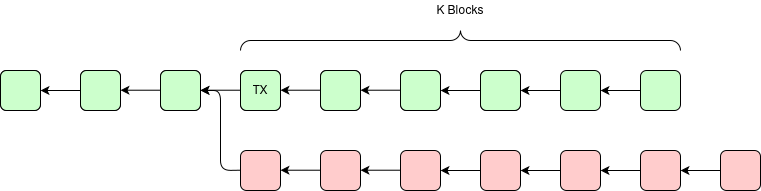
\includegraphics[width=0.85\textwidth]{attack2.png}
	\caption{a successful attack needs to create a longer chain that does not contain the transaction TX}
\end{figure}

Let's suppose an attacker wants to get an item for free. The attacker would fist purchase the item, then wait for K blocks to be appended to the chain so that the transaction is confirmed. After receiving the item, the attacker would then try to fork the chain with blocks that does not contain the transaction. If the new chain becomes the longest, then the attacker would have essentially reversed the transaction and got the item for free. However, with the mining puzzle, this is really hard. Attacker would have to mine K more blocks than the honest nodes in a short time window. Since the probability of solving the puzzle is proportional to the computational power, the attacker would need to have more computational power than the computational power of all honest nodes combined.


\section{Nakamoto Consensus Algorithm}
Regarding Nakamoto's Blcokchain Implementation, the following a few rules must be observed
\begin{itemize}
    \item Each node always tries to mine transaction blocks off the \textbf{Longest Valid Chain}.
    \item When a new block is mined, the miner node must append it to others.
    \item When a host node receives a fresh message or transaction in round $r$, it must echo the message or transaction and all honest node will have observed it by round $r + \Delta$.
\end{itemize}
\subsection{Detailed Algorithm}
\begin{enumerate}
    \item A new node decide to participate and it starts from the initial chain's genesis block
    \begin{itemize}
        \item $chain := (0, 0, \perp, H(0, 0, \perp))$
    \end{itemize}
    \item Whenever a node receives a message $chain'$ from the network, the node will validate the chain and replace the known chain if needed.
    \begin{itemize}
        \item if $valid(chain') \wedge ( |chain'| > |chain| ) \longmapsto chain := chain'$ 
    \end{itemize}
    \item In each round, all nodes try to mine a block from the longest chain.
    \begin{itemize}
        \item Previous chain is denoted as $chain[-1] := (\_, \_, \_, h_{-1})$
        \item A new $txs$ is picked from the transaction pool
        \item A Difficulty Dynamic Parameter, $D_p$, is set for this round
        \item A random seed $y \in \{0, 1\}^{\lambda}$ is picked to compute the hash $h = H(h_{-1}, y, txs)$
        \begin{itemize}
            \item if $h < D_p$, append the newly minded block $(h_{-1}, y, txs, h)$ to the chain and broadcast $chain||(h_{-1}, y, txs, h)$
            \item else, go back to $step 1$ and try again
        \end{itemize}
    \end{itemize}
    \item $chain[: -K]$ is considered as final
    \begin{itemize}
        \item For example, the longest chain that a node observed so far removing the last $K$ blocks, for which $K$ is set as sufficiently large to maintain consistency
    \end{itemize}
\end{enumerate}

\section*{References}
\beginrefs
\bibentry{1} 
``The computational power in Bitcoin''
{\it https://bitinfocharts.com/comparison/bitcoin-hashrate.html}
\endrefs

% **** THIS ENDS THE EXAMPLES. DON'T DELETE THE FOLLOWING LINE:
\end{document}
